% What does this text have to do with the oracular query that this
% section introduces???  You have to explain the most salient features
% of the section -- like the title -- before diving into details!  -Scott
%
% The main complaint about patent search is an
% insufficient match between the content of patent queries and
% relevant
% patents\cite{lupu2013patent}\cite{magdy2012toward}. However,
% considering the size of a patent query (usually thousand of words),
% the intuition is that there are enough terms to match the relevant
% patents.

In this section we seek to understand the adequacy of the baseline
\emph{Patent Query} as well as an upper bound on performance of the
BM25 and LM models and the sufficiency of terms in the reference patent 
by developing an \emph{Oracular Query}.

\subsection{Oracular Query Formulation}

% As noted previously, I would be careful calling this ``relevance feedback''
% and especially abbreviating it RF since RF usually has a different definition
% based on a vector space or other model.  I would call it AvgRelDiff or
% something similar.  -Scott
We begin by defining an oracular relevance feedback system, which
extracts terms from the judged relevant documents.  To this end, we
calculate a relevance feedback ($\mathit{RF}$) score for each term in the top-100
retrieved documents as follows:
% Use \mathit{RF}, \mathit{Rel}, etc. for multiletter names, 
% otherwise RF is technically R*F!  Fix.  -Scott
\begin{equation}
RF(t,Q)=Rel(t)-Irr(t) 
 \label{eq:score}
\end{equation}\vspace*{-5ex}
\begin{displaymath}t\in \lbrace \mbox{terms in top-100 retrieved documents}\rbrace\end{displaymath}
where $ Rel(t) $ is the average term frequency in retrieved relevant patents and $ Irr(t) $ is the average term frequency in retrieved irrelevant patents. We assume that words with a positive score are {\em useful words} since they are more frequent in relevant patents, while words with negative score are {\em noisy words} as they appear more frequently in irrelevant patents.  We seek to evaluate the optimal threshold $\tau$ empirically.

% Huh??? -Scott
%
%We expected to see a higher performance for the queries which contain more {\em useful words}, but, surprisingly, we could not find any correlation between the performance and the presence of {\em useful words} in the query. 

%We hypothesized that a query, formulated by only the {\em useful terms}, is the best possible query we can make since they are all frequent in relevant patents but rare in irrelevant ones. 
We formulate two oracular queries. The first query is formulated by positive terms in top-100 documents as follows: 
\begin{equation}
Oracular \; Query = \{t \in \mathrm{top-100}|RF(t, Q)>\tau\}   
 \label{eq:score}
\end{equation}
We formulate the second query by selecting only {\em useful terms} inside the reference patent:
% query based on the hypothesis that a patent query contains sufficient words matched with the relevant patents:
\begin{equation}
 Oracular \; Patent \; Query = \{t\in Q|RF(t, Q)>\tau\}   
 \label{eq:score}
\end{equation}
%The system performance to these two queries were encouraging. We discuss the detailed results in the next section.

\subsection{Baseline vs. Oracular Query}

%%%%%%%%%%%%%%%%%%%%%%%%%%%%%%%%%%%%%%%%%%%%%%%%%%%%%%%%%%%%%%
\begin{figure}[t!]
\begin{centering}
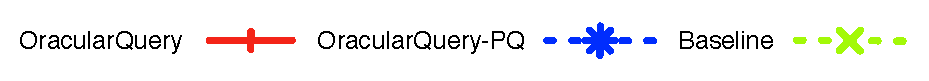
\includegraphics[width=9cm]{imgs/legend}
\par\end{centering}

\begin{centering}
\subfigure[{Mean Average Precision.}]{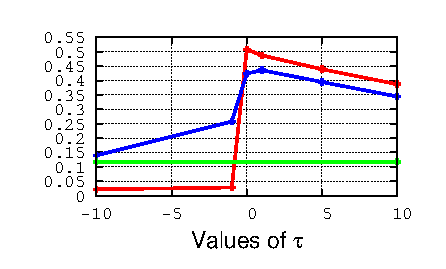
\includegraphics[width=4.5cm]{imgs/figure1-MAP}}\subfigure[Recall.]{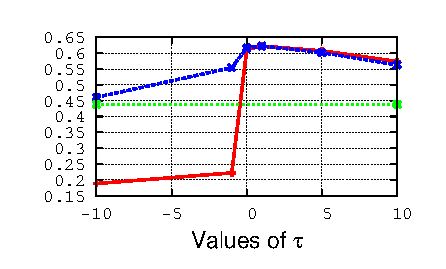
\includegraphics[width=4.5cm]{imgs/figure1-Recall}}
\par\end{centering}

\protect\caption{System performance vs. the threshold $\tau$ for oracular query and oracular patent query.}
\label{fig:oracular}
\end{figure}
%%%%%%%%%%%%%%%%%%%%%%%%%%%%%%%%%%%%%%%%%%%%%%%%%%%%%%%%%%%%%%

First we investigate the ideal threshold setting $\tau$.
Figure \ref{fig:oracular} illustrates that $\tau=0$ is the
best-performing value for {\em Oracular Query} while $\tau=1$ is the
best for {\em Oracular Patent Query}.  The MAP and the recall for the {\em Oracular
Patent Query} are lower than the MAP and the recall for the {\em Oracular Query} respectively;
nonetheless the terms selected from the reference patent itself are
still sufficient to achieve performance significantly better than the
Top CLEF-IP 2010 result.  In addition, we remark on the rather
unexpected steep drop-off in performance when the oracular query
includes slightly noisy terms (i.e., $tau$ just slightly less than 0)
as defined previously.

% What is the ``Best Run''???  You cannot make up words and expect the
% reader to understand.  Be precise on the first introduction that
% this is the best result from CLEF-IP 2010 and provide a citation.
% And call it the ``Top CLEF-IP 2010'' system to be crystal clear.
% Furthermore, it has been mentioned previously that the MAP from CLEF-IP 2010
% and the MAP you provide are not directly comparable since some topics are
% excluded from this evaluation --- for full disclosure you need to explain
% all details of how these MAP measurements differ (and hence indicate this
% Top CLEF-IP 2010 result is only included for a rough comparison of
% performance).  Fix all of these issues and all name changes resulting
% from these updates.  -Scott
%
% Update this discussion with the new table contents.  -Scott
%
% Also, streamline the text... so many sentences are redundant or 
% unneccessary!  You're not done writing until you've removed every
% word possible without changing the meaning of what's written.  -Scott
%
% If different \tau's were used then be clear on this, or simply mention
% Oracular Patent Query $\tau=1$ in the table entry and mention in the
% text how this optimal \tau was selected.  Maybe Figure 1 should come
% before Table 1?  This would better explain how the best \tau's were
% selected.  -Scott
%

%%%%%%%%%%%%%%%%%%%%%%%%%%%%%%%%%%%%%%%%%%%%%%%%%%%%%%%%%%%%%%
\begin{table*}[t!]
  \begin{center}
   \caption{Performance for the {\em Patent Query}, two variants of the {\em Oracular Query}, and {\em Top CLEF-IP 2010}.}
   \vspace*{1ex}
  \input table/optquery.tex   
  \label{tab:optquery}
  \end{center}  
\end{table*}
%%%%%%%%%%%%%%%%%%%%%%%%%%%%%%%%%%%%%%%%%%%%%%%%%%%%%%%%%%%%%%

In Table~\ref{tab:optquery}, we compare our two oracular relevance
queries with both the baseline \emph{Patent Query} and the \emph{Top
CLEF-IP 2010} system~\cite{lopez2010experiments}.  Here we see that
the {\em Oracular Query} using $\tau=0$ far outperforms the baseline and
approximately performs twice as well on MAP as the best competitor in
CLEF-IP 2010.

%
% Unweighted is most natural so no need to even mention it.  -Scott
%
%We observed that a weighed --by query term
%frequency-- query performs better than the unweighed one. However, our
%oracular query performed better unweighed, so, we compare the results
%with unweighed baseline query. The {\em best run} in CLEF-IP 2010
%achieved 0.27 MAP~\cite{lopez2010experiments}.

%Next, we used a threshold $\tau$ to formulate the {\em Oracular Query}
%and {\em Oracular Patent Query} to include merely terms with the RF
%score higher than $\tau$ ($RF(t,Q)>0$).

% Good: is space allows, the enumeration helps make the take-home points
% of this section clear for the reader and leads into the next section.  -Scott
Overall, our experiments related to oracular relevance feedback system
suggest two important conclusions: (1) Query reduction should suffice for effective prior art patent retrieval; and (2) Very precise methods for eliminating poor query terms in the reduction process.


